% !TEX program = pdflatex
\documentclass[aspectratio=169, 11pt]{beamer}

\usetheme{default}
\usecolortheme{default}
\setbeamertemplate{navigation symbols}{}
\setbeamertemplate{footline}[frame number]
\setbeamertemplate{frametitle}{\vspace{0.5em}\textbf{\insertframetitle}}

\usepackage{amsmath,amssymb}
\usepackage{graphicx}
\usepackage{booktabs}
\usepackage{colortbl}
\usepackage{xcolor}
\usepackage{pgfpages}

% Speaker notes on right side
\setbeameroption{show notes on second screen=right}

\graphicspath{{../}}

\definecolor{resultbg}{HTML}{E8F5E9}
\definecolor{highlight}{HTML}{1565C0}

\title{Week 2 Update}
\author{Michael Fang}
\date{March 2026}

\begin{document}

%----------------------------------------------------------------------
\begin{frame}
\centering
\vspace{2em}
{\Large\textbf{Week 2 Update}}

\vspace{1em}
Michael Fang

\vspace{0.5em}
March 2026
\end{frame}
\note{
Weekly progress meeting with Professor Torquato.

Main things to cover:
\begin{itemize}
  \item What I finished from last week
  \item New patterns I analyzed (Classes II, III)
  \item The Bombieri-Taylor result
  \item Updated ranking
\end{itemize}
}

%----------------------------------------------------------------------
\begin{frame}{Quick Recap: What I Had Last Week}

Last week I had:
\begin{itemize}
    \item Variance code validated (Poisson benchmark, 1.1\% error)
    \item Three metallic-mean chains: Fibonacci, Silver, Bronze
    \item All gave $\alpha = 3$ as expected
\end{itemize}

\vspace{0.5em}
\begin{table}
\centering
\begin{tabular}{lccc}
\toprule
\textbf{Pattern} & $\boldsymbol{\alpha}$ (measured) & $\boldsymbol{\alpha}$ (expected) & $\boldsymbol{\bar{\Lambda}}$ \\
\midrule
Fibonacci & 3.05 & 3 & 0.200 \\
Silver & 2.99 & 3 & 0.250 \\
Bronze & 2.99 & 3 & 0.282 \\
\bottomrule
\end{tabular}
\end{table}

\vspace{0.5em}
\textbf{This week:} I wanted to cover all three hyperuniformity classes and find something in the $1 < \alpha < 2$ gap.
\end{frame}
\note{
Quick reminder of where we left off.

The metallic means all give $\alpha = 3$ because of the 2x2 matrix constraint: $|\lambda_2| = 1/|\lambda_1|$.

Goal this week was to expand beyond just $\alpha = 3$.
}

%----------------------------------------------------------------------
\begin{frame}{Class II: Period-Doubling}

I implemented the Period-Doubling chain:
\[
S \to L, \quad L \to LSS \qquad \Rightarrow \qquad M = \begin{pmatrix} 0 & 2 \\ 1 & 1 \end{pmatrix}
\]

\vspace{0.5em}
Matrix gives $\lambda_1 = 2$, $|\lambda_2| = 1$

\vspace{0.3em}
So: $\displaystyle\alpha = 1 - \frac{2\ln(1)}{\ln(2)} = 1$

\vspace{0.5em}
\textbf{What I found:}
\begin{itemize}
    \item Variance grows like $\ln R$ (not bounded, not power-law)
    \item $\bar{\Lambda}$ diverges --- can't use it to rank this pattern
    \item This is the boundary case: $\alpha = 1$ exactly
    \item \colorbox{resultbg}{Class II confirmed}
\end{itemize}
\end{frame}
\note{
Period-Doubling is the boundary case: $\alpha = 1$ exactly.

$|\lambda_2| = 1$ means $\ln(1) = 0$ in the formula.

This is our first Class II example --- variance grows logarithmically.
}

%----------------------------------------------------------------------
\begin{frame}{Class III: 0222 Chain}

Also implemented the 0222 chain:
\[
S \to LL, \quad L \to SSLL
\]

\begin{columns}[T]
\begin{column}{0.45\textwidth}
\vspace{0.5em}
Here $|\lambda_2| = \sqrt{5} - 1 > 1$

So: $\alpha \approx 0.64$

\vspace{0.5em}
\textbf{What I found:}
\begin{itemize}
    \item Variance grows like $R^{0.36}$
    \item $\bar{\Lambda}$ diverges
    \item Class III confirmed
\end{itemize}

\vspace{0.5em}
Now I have examples of all three classes.
\end{column}

\begin{column}{0.55\textwidth}
\centering
\small
\textbf{The three classes:}
\vspace{0.3em}

\begin{tabular}{lcc}
\toprule
\textbf{Class} & $\boldsymbol{\alpha}$ & $\boldsymbol{\sigma^2(R)}$ \\
\midrule
I & $> 1$ & bounded \\
II & $= 1$ & $\sim \ln R$ \\
III & $< 1$ & $\sim R^{1-\alpha}$ \\
\bottomrule
\end{tabular}

\vspace{1em}
The exponent $1 - 0.64 = 0.36$ matches what I measured.
\end{column}
\end{columns}
\end{frame}
\note{
0222 has $|\lambda_2| > 1$, which gives $\alpha < 1$.

The power-law growth $R^{0.36}$ matches the prediction $R^{1-\alpha}$.

Now we have all three classes covered.
}

%----------------------------------------------------------------------
\begin{frame}{URL Verification}

I also tested the perturbed lattice formula you mentioned:
\[
\bar{\Lambda}(a) = \frac{1}{6} + \frac{a^2}{3}
\]

\begin{columns}[T]
\begin{column}{0.45\textwidth}
\vspace{0.5em}
\textbf{My numerical results:}
\begin{center}
\begin{tabular}{ccc}
\toprule
$a$ & Numerical & Exact \\
\midrule
0.1 & 0.168 & 0.170 \\
0.5 & 0.208 & 0.208 \\
1.0 & 0.334 & 0.333 \\
\bottomrule
\end{tabular}
\end{center}

\vspace{0.3em}
Errors $< 0.3\%$ --- this validates my code against an independent analytical result.
\end{column}

\begin{column}{0.55\textwidth}
\centering
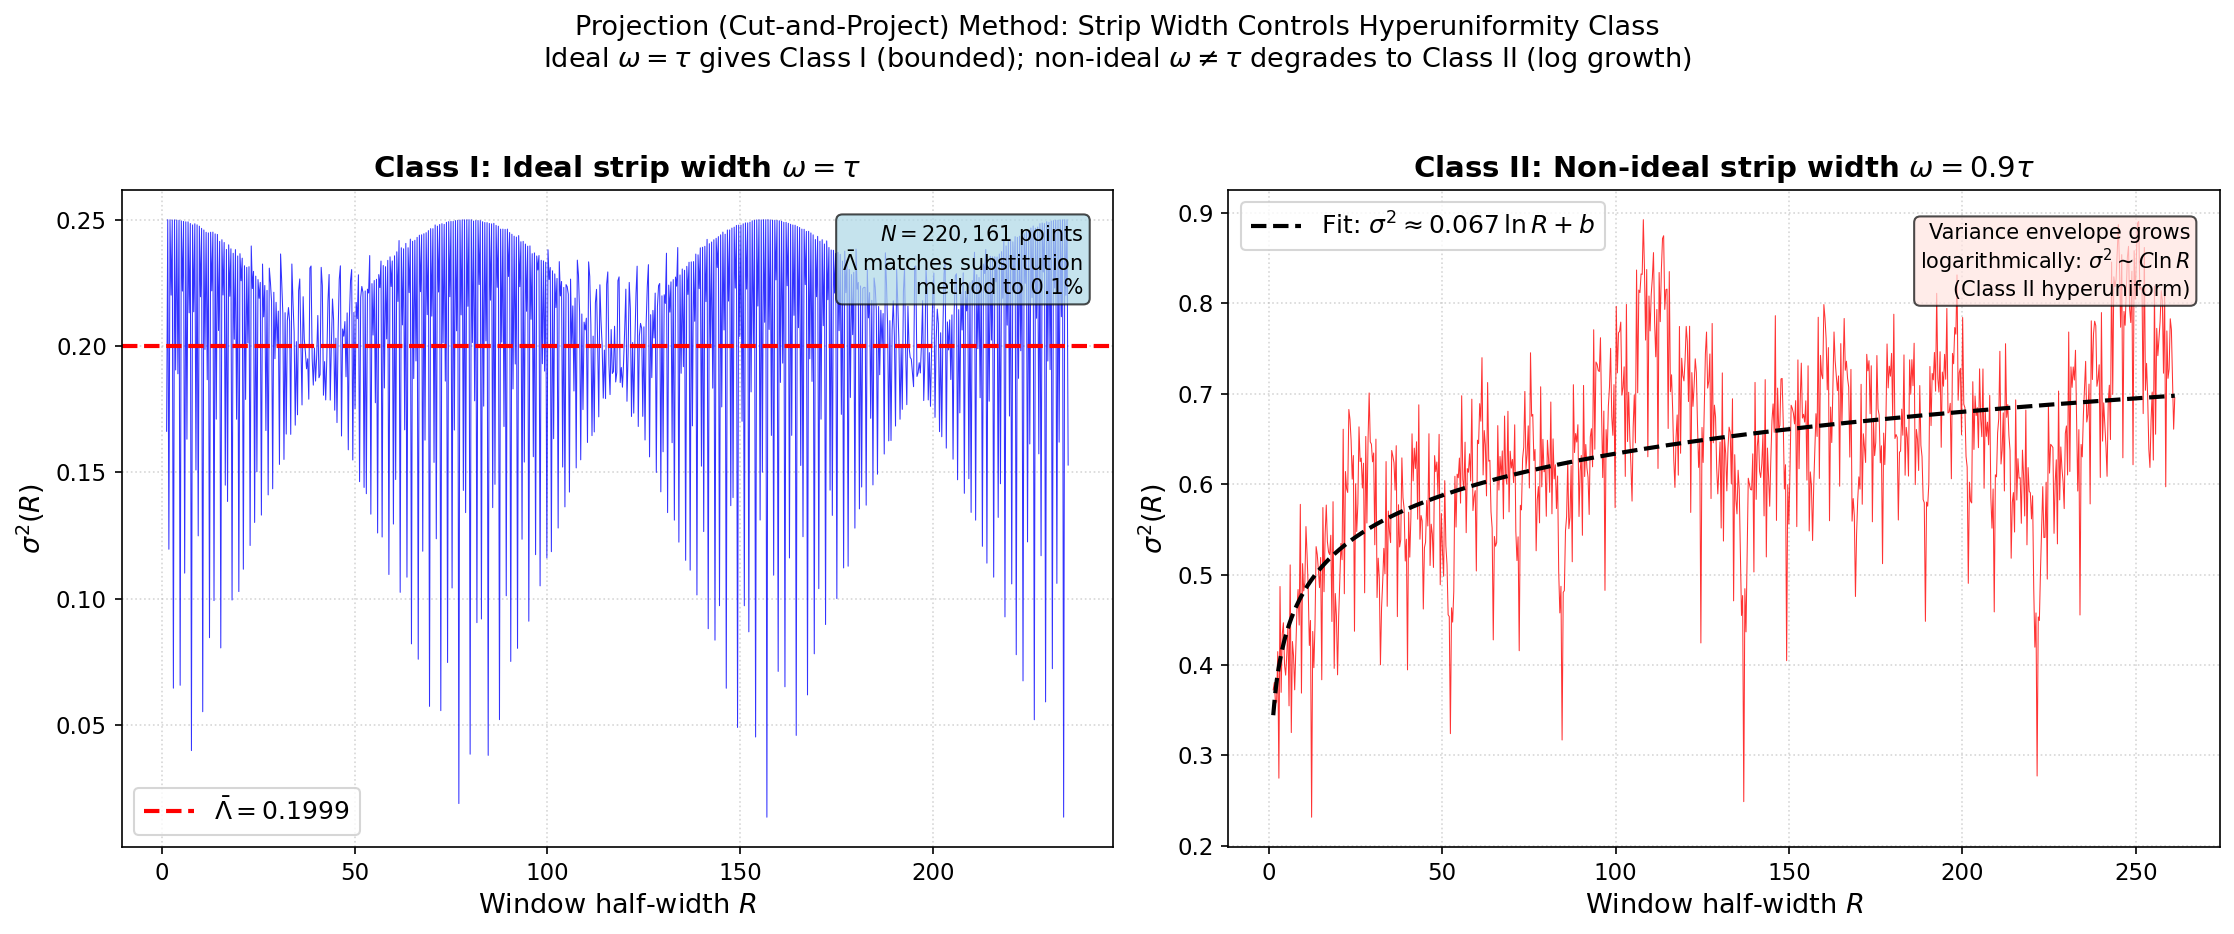
\includegraphics[width=\linewidth]{fig4_projection_comparison.png}
\end{column}
\end{columns}
\end{frame}
\note{
URL = uncorrelated random lattice (independent displacements).

Good validation because we have the exact formula.

Always $\alpha = 2$ regardless of displacement amplitude $a$.
}

%----------------------------------------------------------------------
\begin{frame}{Stealthy Patterns}

I analyzed stealthy configurations provided by another group member.

\vspace{0.3em}
\textbf{Idea:} Force $S(k) = 0$ for all $|k| < K^*$, not just at $k = 0$.

\vspace{0.5em}
\textbf{Results} ($N = 2{,}000$, $\sim$4000 configs each):
\begin{center}
\begin{tabular}{ccc}
\toprule
$\chi$ & $\bar{\Lambda}$ & $\alpha$ \\
\midrule
0.1 & 0.166 & 2.0 \\
0.2 & 0.166 & 2.0 \\
0.3 & 0.166 & 2.0 \\
\bottomrule
\end{tabular}
\end{center}

\vspace{0.5em}
\textbf{Key observation:} $\bar{\Lambda} \approx 1/6$ --- same as the perfect lattice!

\vspace{0.3em}
These disordered patterns achieve optimal hyperuniformity.
\end{frame}
\note{
Data from another grad student (CCO format, ~4000 configs per $\chi$).

$\chi$ controls the size of the exclusion region.

Remarkable: disordered patterns achieve lattice-level $\bar{\Lambda}$.
}

%----------------------------------------------------------------------
\begin{frame}{The Gap Problem}

At this point I noticed a gap in my data:

\vspace{0.3em}
\begin{center}
\begin{tabular}{lcl}
\toprule
$\alpha$ & Class & What I have \\
\midrule
3 & I & Fibonacci, Silver, Bronze \\
2 & I & URL, Stealthy \\
\rowcolor{yellow!30}
$1 < \alpha < 2$ & I & \textcolor{red}{Nothing!} \\
1 & II & Period-Doubling \\
$< 1$ & III & 0222 \\
\bottomrule
\end{tabular}
\end{center}

\vspace{0.5em}
The problem: all 2$\times$2 metallic-mean matrices give $\alpha = 3$ because $|\lambda_2| = 1/|\lambda_1|$.

\vspace{0.3em}
You suggested looking at the Bombieri-Taylor cubic substitution from their 1986 paper.
\end{frame}
\note{
The 2x2 constraint: det$(M) = \pm 1$ forces $|\lambda_2| = 1/|\lambda_1|$.

This always gives $\alpha = 1 + 2 = 3$.

Need a 3x3 matrix to break this constraint.
}

%----------------------------------------------------------------------
\begin{frame}{Bombieri-Taylor Cubic Substitution}

From the 1986 paper (p. C3-21):

\begin{columns}[T]
\begin{column}{0.45\textwidth}
\vspace{0.3em}
\textbf{Three-letter alphabet:}
\[
a \to aac, \; b \to ac, \; c \to b
\]

\textbf{Matrix:}
\[
M = \begin{pmatrix} 2 & 0 & 1 \\ 1 & 0 & 1 \\ 0 & 1 & 0 \end{pmatrix}
\]

Eigenvalues: $\theta_1 = 2.247$, $|\lambda_2| = 0.802$
\end{column}

\begin{column}{0.55\textwidth}
\textbf{Predicted:}
\[
\alpha = 1 - \frac{2\ln(0.802)}{\ln(2.247)} = \colorbox{resultbg}{\textbf{1.545}}
\]

\vspace{0.5em}
\textbf{What I did:}
\begin{itemize}
    \item Extended my code for 3-letter alphabets
    \item Generated 9.5 million points
    \item Computed variance and $\bar{\Lambda}$
\end{itemize}

\vspace{0.5em}
\textbf{Result:} $\bar{\Lambda} = 0.377$, Class I confirmed.
\end{column}
\end{columns}
\end{frame}
\note{
Key: $|\lambda_2| = 0.802 \neq 1/\theta_1 = 0.445$.

The 3x3 matrix breaks the constraint!

$\theta_1$ is a Pisot number (conjugates all $< 1$).
}

%----------------------------------------------------------------------
\begin{frame}{Bombieri-Taylor Results}
\centering

\includegraphics[width=0.78\linewidth]{bombieri_taylor_analysis.png}

\vspace{0.2em}
\small
Variance is bounded (Class I). The log-periodic oscillations in spreadability are expected for quasicrystals.
\end{frame}
\note{
Panel (a): Bounded variance confirms Class I.

Panel (c): Log-periodic oscillations with period $\ln(\theta_1)$.

Panel (d): Shows where B-T fits in the ranking.

The eigenvalue formula $\alpha = 1.545$ is exact.
}

%----------------------------------------------------------------------
\begin{frame}{Updated Ranking}

Here's where everything stands now:

\vspace{0.3em}
\centering
\begin{tabular}{lccc}
\toprule
\textbf{Pattern} & \textbf{Class} & $\boldsymbol{\alpha}$ & $\boldsymbol{\bar{\Lambda}}$ \\
\midrule
Lattice & I & $\infty$ & 0.167 \\
Stealthy & I & 2.0 & 0.166 \\
URL ($a=0.1$) & I & 2.0 & 0.168 \\
Fibonacci & I & 3.0 & 0.200 \\
Silver & I & 3.0 & 0.250 \\
Bronze & I & 3.0 & 0.282 \\
URL ($a=1.0$) & I & 2.0 & 0.333 \\
\rowcolor{resultbg}
\textbf{Bombieri-Taylor} & \textbf{I} & \textbf{1.545} & \textbf{0.377} \\
\midrule
Period-Doubling & II & 1.0 & diverges \\
0222 & III & 0.64 & diverges \\
\bottomrule
\end{tabular}
\end{frame}
\note{
26 patterns total now (counting different $\chi$ and $a$ values).

Bombieri-Taylor fills the gap between $\alpha = 1$ and $\alpha = 2$.

This is the first quasicrystal I know of with $1 < \alpha < 2$.
}

%----------------------------------------------------------------------
\begin{frame}{Summary}

\textbf{What I did this week:}
\begin{itemize}
    \item Added Class II (Period-Doubling, $\alpha = 1$)
    \item Added Class III (0222, $\alpha = 0.64$)
    \item Verified URL formula to $< 0.3\%$
    \item Generated stealthy patterns ($\bar{\Lambda} \approx 1/6$)
    \item Implemented Bombieri-Taylor cubic ($\alpha = 1.545$)
\end{itemize}

\vspace{0.5em}
\textbf{Main result:} Filled the $1 < \alpha < 2$ gap with a quasicrystal.

\vspace{0.5em}
\textbf{Questions for you:}
\begin{itemize}
    \item Are there other cubic/quartic substitutions I should try?
    \item Should I look at 2D generalizations next?
\end{itemize}
\end{frame}
\note{
Total patterns analyzed: 26

Key accomplishment: Bombieri-Taylor fills the gap.

Possible next steps: other cubic substitutions, 2D/3D.
}

%----------------------------------------------------------------------
\begin{frame}{References}

\small
\begin{itemize}
    \item Torquato \& Stillinger (2003), Phys. Rev. E 68, 041113
    \item Bombieri \& Taylor (1986), J. Physique Colloques 47, C3-19
    \item O\u{g}uz et al. (2017), Phys. Rev. B 95, 054119
    \item Torquato (2021), Phys. Rev. E 104, 054102
\end{itemize}
\end{frame}
\note{
Main references used this week.
}

\end{document}
